\textbf{Συνοπτική περιγραφή των τεχνικών χαρα\-κτη\-ρι\-στικών του motion capture με χρήση drone swarm συστήματος, που σχετίζεται η παραπάνω διπλωματική.}
  
%%%%%%%%%%%%%%%%%%%%%%%%%%%%%%%%%%%%%%%%%%%%%%%%%%%%%%%%%%%%%%%%%%%%%%%%%%%%%%%%

\section{Hardware}
Σε πρώτο στάδιο το Embedded Linux System στο οποίο επιλέχθηκε να γίνει η ανάπτυξη, είναι το Raspberry Pi 4 Model B - Table \ref{tab:1} - έναντι κάποιου board της οικογένειας Jetson, λόγω του ότι αποτελεί μία ελάχιστα οικονομικότερη καθώς και σε βάρος ελαφρότερη επιλογή. Όπως αναφέρθηκε και στο thesis proposal, εάν κριθεί όμως αναγκαίο (εξαιτίας του online onboard image processing που πραγματοποιείται) θα γίνει migration ενός ή περισσότερων κόμβων του συστήματος σε Jetson. 

\begin{table}[H]
  \caption[]{Raspberry Pi 4 Model B Specifications}
  \label{tab:1}
  \centering
  \begin{tabular}{ll}
      \hline
      \textbf{Feature} & \textbf{Value}  \\
      \hline
          Processor & \Centerstack{Broadcom BCM2711, Quad core Cortex-A72 \\(ARM v8) 64-bit SoC @ 1.5GHz }\\
          Memory & 8GB LPDDR4-3200 SDRAM \\
          Storage & External Micro-SD \\  
          Power & 5V DC (maximum 3A), 5-15Watt \\
          Weight & 46 grams (without case), 99 grams (with case) \\
          Peripherals & GPIO, I2C, SPI, UART \\
          \hline
  \end{tabular}
\end{table}

\subsection{Components}
Στο Table \ref{tab:2} παρουσιάζονται τα ακριβή components τα οποία επιλέχθηκαν για τα πρώτα στάδια σχεδιασμού του συστήματος και τους αρχικούς ελέγχους ορθής λειτουργίας, καθώς και το κόστος του καθενός από αυτά.  

\begin{table}[H]
  \caption[]{Bill of Materials}
  \label{tab:2}
  \centering
  \begin{tabular}{ll}
      \hline
      \textbf{Component} & \textbf{Cost}  \\
      \hline
          Raspberry Pi 4 Model B 8GB & \Centerstack{$\sim$ 100 €}\\
          Creative live cam sync 1080p \cite{creative-camera} & \Centerstack{$\sim$ 44 €}\\
          BN-220 GPS Module \cite{bn-220-gps} & \Centerstack{$\sim$ 15 €}\\
          Adafruit 10 DoF IMU \cite{adafruit-10dof-imu} & \Centerstack{$\sim$ 30 €}\\
          Breakout Board with fan \cite{raspberry-pi-fan-breadkout} & \Centerstack{$\sim$ 8 €}\\
          \hline
  \end{tabular}
\end{table}

\section{Software}
Σχετικά με το λειτουργικό σύστημα, χρησιμοποιείται η έ\-κδο\-ση Ubuntu 20.04.2 64bit version για ΑRM \cite{ubuntu-raspberry} η οποία είναι σχεδιασμένη ειδικά για το Raspberry Pi. Στο οποίο εγκαταστάθηκε η έκδοση noetic του Robot Operating System (ROS)\cite{Ros-noetic-installation}.

\subsection{ROS packages}
Για να μπορούν τα components που αναφέρθηκαν παραπάνω να λειτουργούν - καθώς και συνολικά το σύστημα - έχουν εγκατασταθεί επίσης τα παρακάτω πακέτα στο ROS.

\newpage

Packages:
\begin{itemize}
  \addtolength{\itemindent}{0.3cm}
  \item tf2\_ros
  \item robot\_localization
  \item usb\_cam
  \item nmea\_navsat\_driver
\end{itemize}

\section{System Overview}
Στο Figure \ref{fig:1} παρουσιάζεται η μορφή του συστήματος μέχρι αυτήν την στιγμή. Το σύστημα ζυγίζει $\sim$ 250gr στο σύνολο του, ενώ μία αρχική εκτίμηση κατανάλωσης είναι περίπου τα 15Watt.

\begin{figure}[thpb]
  \centering
  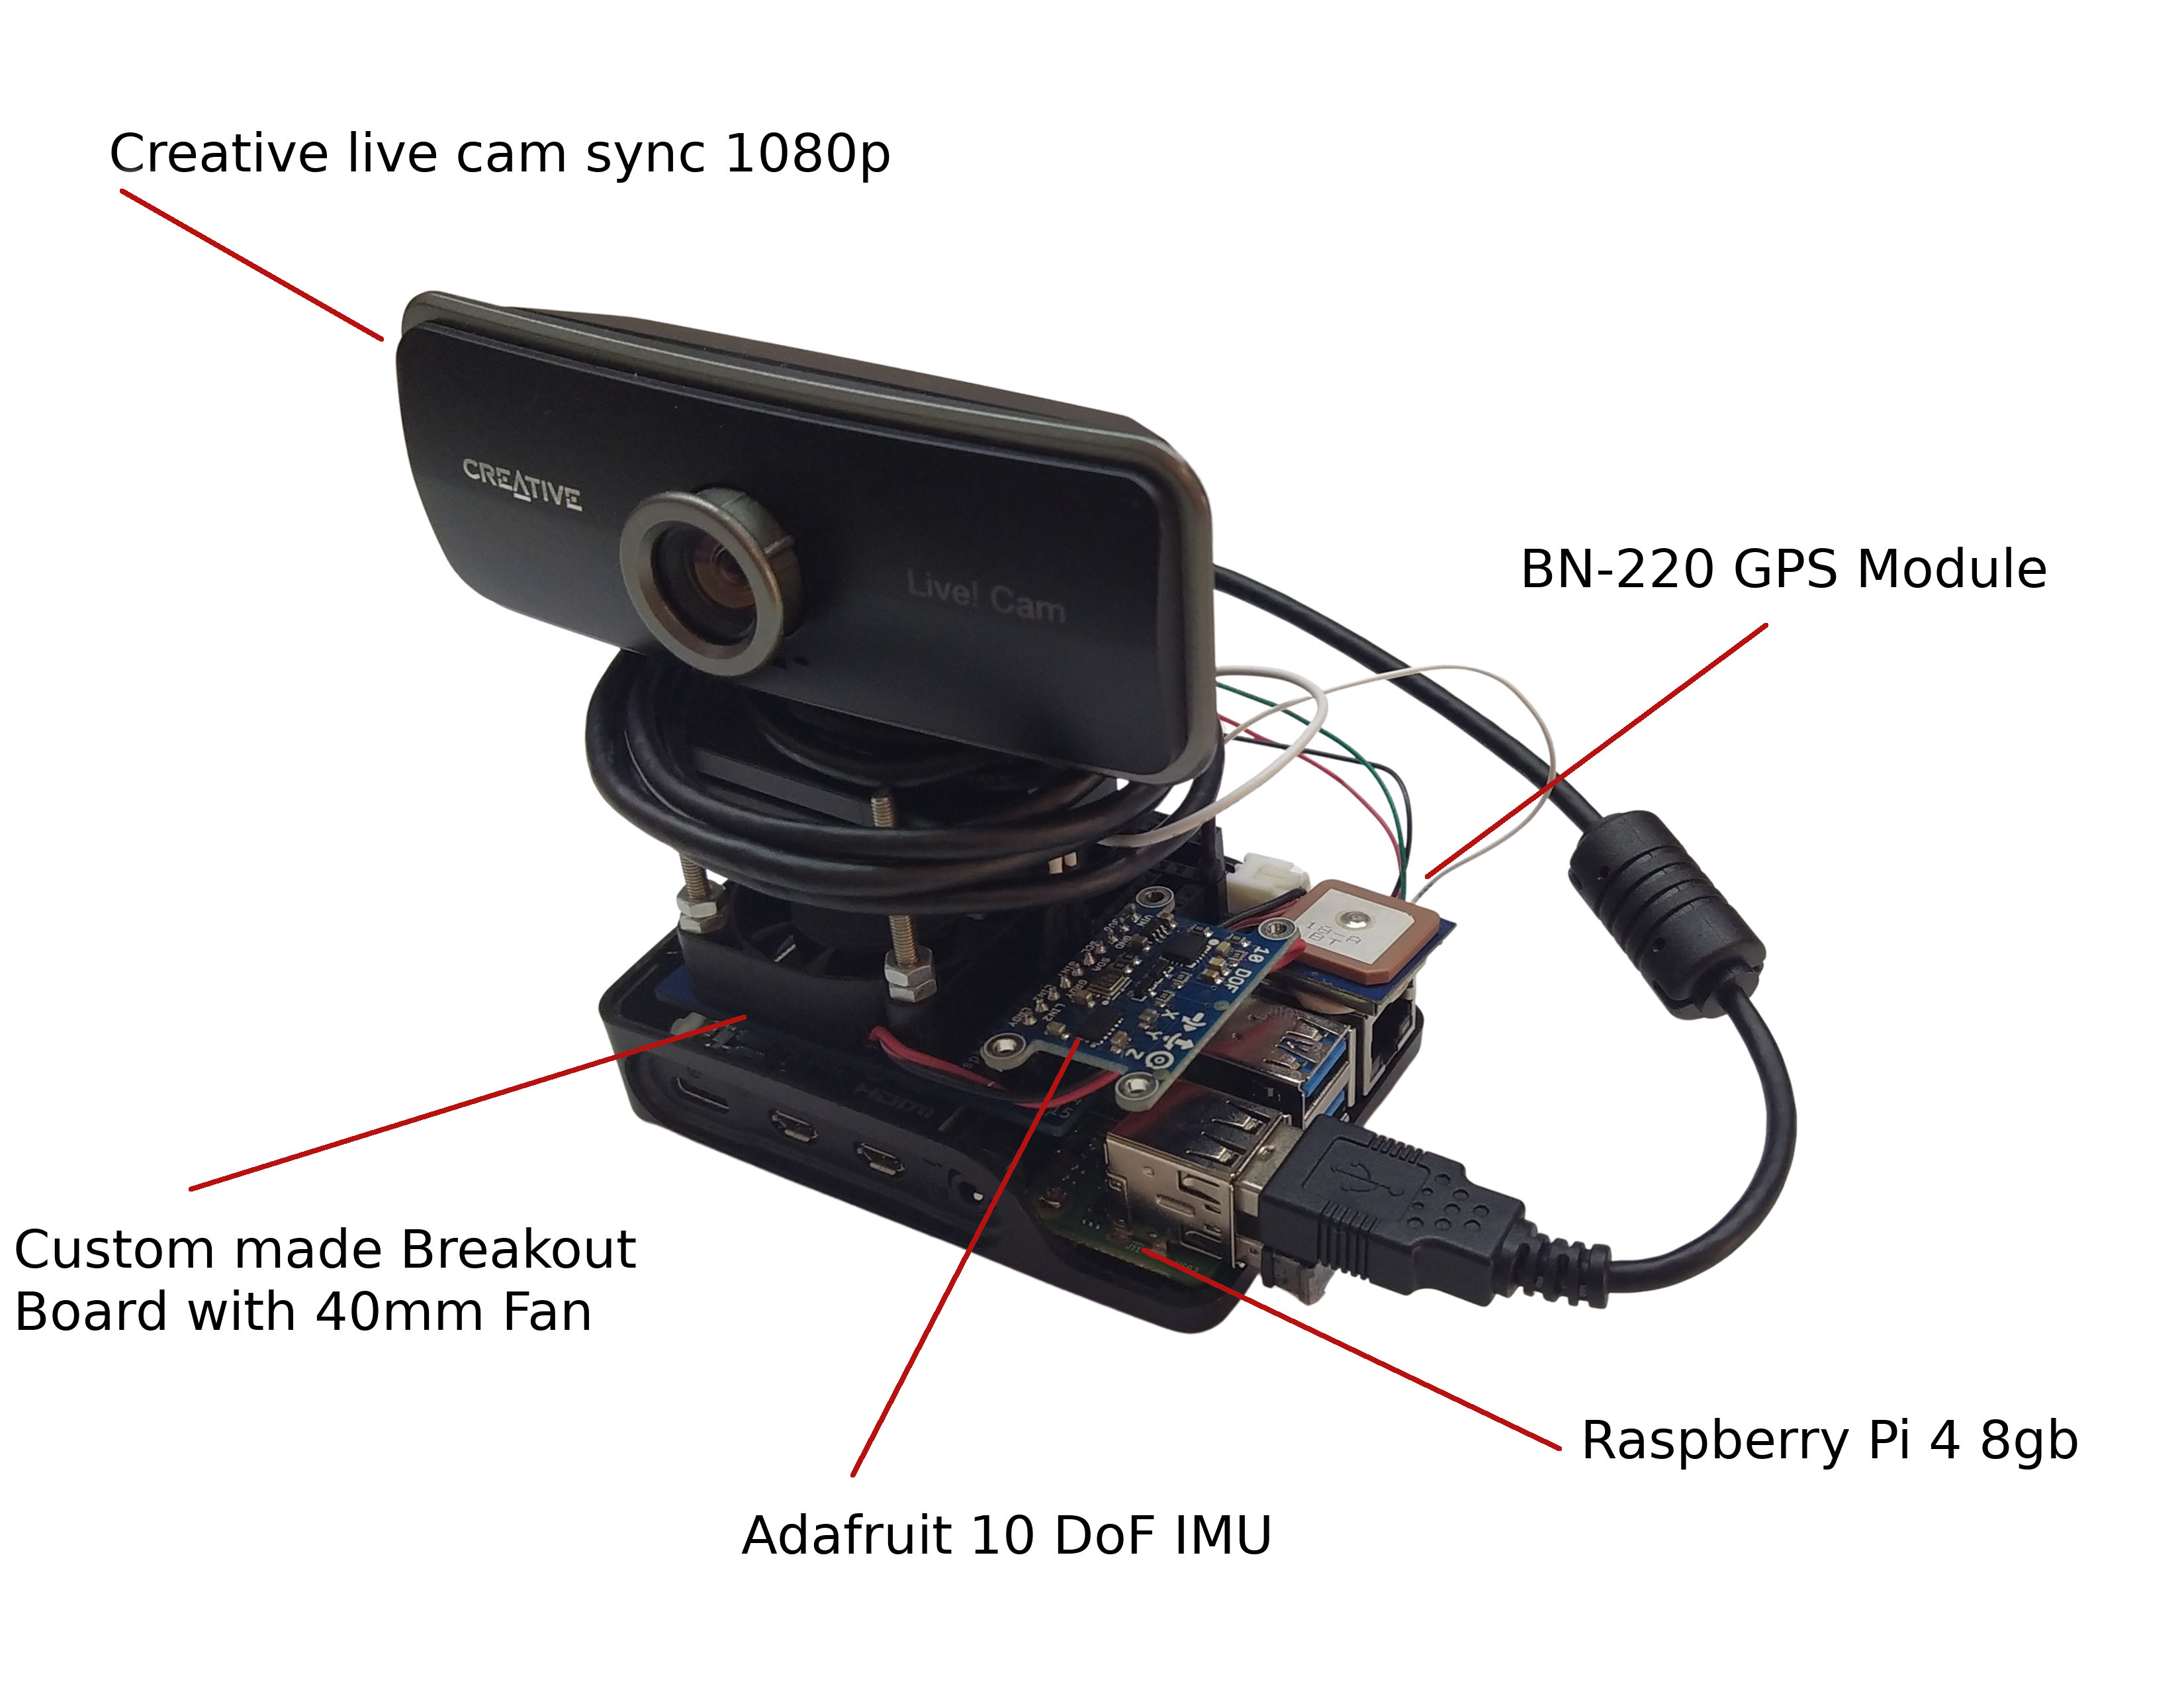
\includegraphics[width=\linewidth]{Images/thesis-system.jpg}
  \caption{Current system }
  \label{fig:1}
\end{figure}




